\chapter{Irraggiamento}

Quando le cariche \emph{accelerano}, i loro campi possono trasportare energia in modo \emph{irreversibile} all'infinito. Questo processo prende il nome di \emph{irraggiamento}. \footnote{In realtà è necessario fare una precisazione. Il termine più corretto da utilizzare sarebbe \emph{irraggiamento all'infinito}, in quanto, nel quotidiano, il termine irraggiamento viene usato (\emph{erroneamente}) riferendosi a una sorgente che emette energia sotto forma di onde elettromagnetiche, ma questa energia non viene necessariamente trasportata all'infinito. \\} \mkeyword{irraggiamento} \\

Più precisamente, diciamo che un sistema irradia quando il flusso del vettore di Poynting attraverso una superficie sferica di raggio $r$ rimane finito e non nullo nel limite $r \to \infty$:

\begin{equation}
    P_{\text{rad}} = \lim_{r \to \infty} \oint \mathbf{S} \cdot d \Sigma \ \mathbf{u}_n \neq 0
\end{equation}

Si nota allora che, dato che l'area è proporzionale a $r^2$, affinché ci sia irraggiamento è necessario che il vettore di Poynting non decada più velocemente di $1/r^2$. \\
Quindi per studiare l'irraggiamento è necessario considerare le parti di $\mathbf{E}$ e $\mathbf{B}$ che decadono come $1/r$ quando siamo in zona di radiazione ($d \ll \lambda \ll r$). \\

Adesso andremo ad analizzare l'irraggiamento di diversi tipi di sorgenti. 

\section{Irraggiamento di una carica puntiforme}

Supponiamo di considerare una carica puntiforme $q$ in moto con traiettoria $\mathbf{r}_q$ e velocità $\mathbf{v}(t) = \dot{\mathbf{r}}_q(t)$. Sappiamo che a questa sono associati i potenziali di Liènard-Wiechert \eqref{eq: potenziali_Liènard-Wiechert}. 
Grazie a questi è possibile ricavare il campo elettrico e il campo magnetico generati dalla carica, i quali risultano essere\footnote{Per vedere come si ricavano formalmente i campi guardare il capitolo 11 di \cite{IntroductiontoElectrodynamics}}:

\begin{tcolorbox}[colback=yellow!10!white, colframe=orange!70!black, boxrule=0.8pt]
\begin{align} 
    \mathbf{E}(\mathbf{r}, t) = \frac{q}{4 \pi \eps_0} \left[\frac{\mathcal{R}}{(\mathbf{\mathcal{R}} \cdot \mathbf{u})^3} \left[(c^2 (1 - \beta^2) \mathbf{u} + \mathbf{\mathcal{R}} \times (\mathbf{u} \times \mathbf{a}))\right] \right]_{\text{rit}} \label{eq: campo_elettrico_carica_moto}\\
    \mathbf{B}(\mathbf{r}, t) = \left[ \frac{1}{c} \hat{\mathcal{R}} \times \mathbf{E} \right]_{\text{rit}} \label{eq: campo_magnetico_carica_moto}
\end{align}
\end{tcolorbox}

\newpage

Dove abbiamo definito 

\begin{align*}
    \boldsymbol{\mathcal{R}} = \mathbf{r} - \mathbf{r}_q(t') \\
    \boldsymbol{\beta} = \frac{\mathbf{v}(t')}{c} \\
    \mathbf{u} = c \hat{\mathcal{R}} - \mathbf{v} = c (\hat{\mathcal{R}} - \mathbf{\beta})\\
    \mathbf{a} = \dot{\mathbf{v}}
\end{align*}

Allora il vettore di Poynting risulta essere 

\begin{equation} \label{eq: Poynting_irr}
    \mathbf{S} = \frac{1}{\mu_0} (\mathbf{E} \times \mathbf{B}) = \frac{1}{\mu_0 c} [\mathbf{E} \times (\hat{\mathbf{\mathcal{R}}} \times \mathbf{E})] = \frac{1}{\mu_0 c}[E^2 \hat{\mathbf{\mathcal{R}}} - (\hat{\mathbf{\mathcal{R}}} \cdot \mathbf{E})\mathbf{E}]
\end{equation}

Tuttavia non dobbiamo considerare tutti i termini del campo elettrico per trovare l'irraggiamento, una parte rappresenta l'energia di campo trasportata dalla particella durante il suo movimento. L'energia irradiata è quella che, di fatto, si \emph{stacca} dalla carica e si propaga all'infinito. \\

Per calcolare la potenza totale irradiata dalla particella al tempo $t_r$, consideriamo una sfera di raggio $\mathcal{R}$ centrata nella posizione della particella al tempo $t_r$. Dato che l'area della sfera è proporzionale a $\mathcal{R}^2$, tutti i termini in $\mathbf{S}$ che vanno come $1/\mathcal{R}^2$ daranno un contributo finito all'irraggiamento, tuttavia i termini come $1/\mathcal{R}^3$ o $1/\mathcal{R}^4$ daranno un contributo nullo per $\mathcal{R} \to \infty$.\\
Per questo \emph{nel campo elettrico solo il termine contenente l'accelerazione contribuisce alla radiazione}. 

\begin{equation}
    \mathbf{E}_{\text{rad}} = \frac{q}{4 \pi \eps_0} \frac{\mathcal{R}}{(\mathbf{{\mathcal{R}}} \cdot \mathbf{u})^3} [\mathbf{\mathcal{R}} \times (\mathbf{u} \times \mathbf{a})]
\end{equation}

Dato che $\mathbf{E}_\text{rad}$ è perpendicolare a $\hat{\mathbf{\mathcal{R}}}$, il secondo termine in \eqref{eq: Poynting_irr} scompare e quindi 

\begin{equation}
    \mathbf{S}_{\text{rad}} = \frac{1}{\mu_0 c} E_{\text{rad}}^2 \hat{\mathbf{\mathcal{R}}}
\end{equation}

Se la carica è istantaneamente a riposo, allora $\mathbf{u} = c \hat{\mathbf{\mathcal{R}}}$ e quindi

\begin{equation}
    \mathbf{E}_{\text{rad}} = \frac{q}{4 \pi \eps_0 c^2 \mathcal{R}} [\hat{\mathbf{\mathcal{R}}} \times (\hat{\mathbf{\mathcal{R}}} \times \mathbf{a})] = \frac{\mu_0 q}{4 \pi \mathcal{R}} [(\hat{\mathbf{\mathcal{R}}} \cdot \mathbf{a}) \hat{\mathbf{\mathcal{R}}} - \mathbf{a}]
\end{equation}

Sostituendo 

\begin{tcolorbox}[colback=yellow!10!white, colframe=orange!70!black, boxrule=0.8pt]
\begin{equation}
    \mathbf{S}_{\text{rad}} = \frac{1}{\mu_0 c} \left( \frac{\mu_0 q}{4 \pi \mathcal{R}} \right)^2 [a^2 - (\hat{\mathbf{\mathcal{R}}} \cdot \mathbf{a})^2] \hat{\mathbf{\mathcal{R}}} = \frac{\mu_0 q^2 a^2}{16 \pi^2 c} \left( \frac{\sin^2(\theta)}{\mathcal{R}^2} \right) \ \hat{\mathbf{\mathcal{R}}}
\end{equation}
\end{tcolorbox}

Allora la potenza totale irradiata è 

\begin{equation}
    P = \oint \mathbf{S}_{\text{rad}} \cdot d \Sigma \ \mathbf{u}_n = \frac{\mu_0 q^2 a^2}{16 \pi^2 c} \int \frac{\sin^2\theta}{\mathcal{R}^2} \mathcal{R}^2 \sin \theta \ d\theta \ d\phi
\end{equation}

La quale può essere scritta come 

\begin{tcolorbox}[colback=yellow!10!white, colframe=orange!70!black, boxrule=0.8pt]
\begin{equation} \label{eq: formula_Larmor}
    P = \frac{\mu_0 q^2 a^2}{6 \pi c}
\end{equation}\
\end{tcolorbox}

Questa è la \emph{formula di Larmor}: \mkeyword{formula di Larmor}qualsiasi carica accelerata irradia energia, con potenza proporzionale al quadrato dell'accelerazione. \\

La formula di Larmor ha implicazioni fisiche profonde: un elettrone classico in orbita attorno a un nucleo è continuamente accelerato centripetamente, quindi dovrebbe irraggiare energia e spiralare verso il nucleo in un tempo brevissimo. 
Questo è uno dei fallimenti fondamentali della fisica classica che ha portato allo sviluppo della meccanica quantistica.\\

Per ricavare questa relazione abbiamo supposto che la carica fosse istantaneamente ferma, tuttavia la \eqref{eq: formula_Larmor} continua a essere valida in buona approssimazione anche quando $v \ll c$. 

\subsection{Forza di reazione di radiazione}

\newpage

\section{Irraggiamento di un dipolo elettrico oscillante}

Consideriamo un dipolo elettrico oscillante. Dato che vogliamo calcolare l'irraggiamento del dipolo, ci interesseranno il campo elettrico e magnetico prodotti dal dipolo \emph{nella zona di radiazione}. 
Nel capitolo precedente abbiamo trovato che questi sono \eqref{eq: E_rad_dipolo} e \eqref{eq: B_rad_dipolo}. \\

Il vettore di Poynting è:

\begin{equation}
    \mathbf{S} = \frac{1}{\mu_0}(\mathbf{E}_{\text{rad}} \times \mathbf{B}_{\text{rad}})
\end{equation}

Per calcolarlo esplicitamente, notiamo che si ha $\mathbf{B}_{\text{rad}} = \frac{1}{c}\hat{r} \times \mathbf{E}_{\text{rad}}$, quindi:

\begin{equation}
    \mathbf{E}_{\text{rad}} \times \mathbf{B}_{\text{rad}} = \mathbf{E}_{\text{rad}} \times \left(\frac{1}{c}\hat{r} \times \mathbf{E}_{\text{rad}}\right) =\frac{1}{c}\left[E_{\text{rad}}^2 \hat{r} - (\mathbf{E}_{\text{rad}} \cdot \hat{r})\mathbf{E}_{\text{rad}}\right]
\end{equation}

Poiché nella zona di radiazione $\mathbf{E}_{\text{rad}} $ è ortogonale a $\hat{r}$ (il campo è trasversale), il secondo termine si annulla e si ottiene:

\begin{tcolorbox}[colback=yellow!10!white, colframe=orange!70!black,boxrule=0.8pt]
\begin{equation} \label{eq: Poynting_radiazione}
    \mathbf{S} = \frac{E_{\text{rad}}^2}{\mu_0 c} \hat{r} = \frac{\mu_0}{16\pi^2 c} \frac{|(\ddot{\mathbf{p}}_r \times \hat{r}) \times \hat{r}|^2}{r^2} \hat{r} = \frac{\mu_0}{16\pi^2 c}\frac{|\ddot{\mathbf{p}}_r |^2 \ \sin^2 \theta}{r^2} \hat{r}
\end{equation}
\end{tcolorbox}

Il vettore di Poynting è diretto radialmente verso l'esterno e decade come $r^{-2}$, garantendo la conservazione dell'energia: il flusso totale attraverso una sfera di raggio $r$ qualsiasi è indipendente da $r$.\\

L'intensità dell'onda, definita come la media sul periodo di $|\mathbf{S}|$, risulta essere 

\begin{tcolorbox}[colback=yellow!10!white, colframe=orange!70!black, boxrule=0.8pt]
\begin{equation}
    I(r,\theta) = \langle |\mathbf{S}| \rangle = \frac{\mu_0 \omega^4 p_0^2 }{32 \pi^2 c} \frac{\sin^2 \theta}{r^2} = \frac{I_0}{r^2} \sin^2 \theta
\end{equation}
\end{tcolorbox}

Dove abbiamo usato il fatto che $\langle \cos^2(\omega t) \rangle = 1/2$ e abbiamo definito 

\begin{tcolorbox}[colback=yellow!10!white, colframe=orange!70!black, boxrule=0.8pt]
\begin{equation}
    I_0 = \frac{\mu_0 p_0^2 \omega^4}{32 \pi^2 c}
\end{equation}
\end{tcolorbox}

Allora possiamo trovare la potenza totale irradiata integrando $I(r, \theta)$ sulla sfera di raggio $r$ (dove $r \to \infty$). 

\begin{equation}
    \langle P \rangle = \oint_{\Sigma} \langle \mathbf{S} \rangle \cdot d\Sigma \ \mathbf{u}_n = \frac{\mu_0 p_0^2 \omega^4}{32 \pi^2 c} \int_{0}^{2\pi} \int_{0}^{\pi} \frac{\sin^2 \theta}{r^2} r^2 \sin \theta \ d\theta \ d \phi = \frac{\mu_0 p_0^2 \omega^4}{12 \pi c}
\end{equation}

E quindi 

\begin{tcolorbox}[colback=yellow!10!white, colframe=orange!70!black, boxrule=0.8pt]
\begin{equation} \label{eq: potenza_dipolo_elettrico}
    \langle P \rangle = \frac{\mu_0 p_0^2 \omega^4}{12 \pi c} = \frac{8 \pi}{3} I_0
\end{equation}
\end{tcolorbox}

\subsection{Potenza irraggiata per unità di angolo solido}

A differenza di quanto abbiamo fatto sopra, adesso non andiamo a considerare tutta la superficie all'infinito, ma solo la parte di superficie $\Sigma$ che sottende un certo angolo solido $\Omega$. Allora si ha 

\begin{equation}
    \frac{d \langle P \rangle}{d \Omega} = \frac{d\langle P \rangle}{d\Sigma} \frac{d\Sigma}{d\Omega}
\end{equation}

Dato che $\Sigma = r^2 \ \Omega$ e $d\langle P \rangle/d\Sigma = I$, si ha

\begin{tcolorbox}[colback=yellow!10!white, colframe=orange!70!black, boxrule=0.8pt]
\begin{equation}
    \frac{d \langle P \rangle}{d \Omega} = I(r, \theta) \ r^2 = \frac{\mu_0 \omega^4 p_0^2}{32 \pi^2 c} \sin^2 \theta  = I_0 \sin^2 \theta
\end{equation}
\end{tcolorbox}

\subsection{Potenza istantanea}

Abbiamo trovato la potenza \emph{media} totale irradiata, tuttavia è possibile trovare anche la potenza \emph{istantanea} totale irradiata.

\begin{equation}
    P(t) = \oint_{\Sigma} \mathbf{S} \cdot d\Sigma \ \mathbf{u}_n = \frac{\mu_0 |\ddot{\mathbf{p}}_r|^2}{16 \pi^2 c} \int_0^{2\pi} \int_{0}^{\pi} \sin^3 \theta \ d\theta \ d\phi = \frac{\mu_0 |\ddot{\mathbf{p}}_r|^2}{6 \pi c} = \frac{\mu_0 p_0^2 \omega^4}{6 \pi c} \cos^2 (\omega t_r)
\end{equation}

Pertanto vale 

\begin{tcolorbox}[colback=yellow!10!white, colframe=orange!70!black, boxrule=0.8pt]
\begin{equation}
    P(t) = \frac{\mu_0 p_0^2 \omega^4}{6 \pi c} \cos^2 (\omega t_r)
\end{equation}
\end{tcolorbox}

Si nota, inoltre, che questo risultato è in perfetto accordo con quello trovato per la potenza media totale, in quanto $\langle \cos^2(\omega t_r)\rangle = 1/2$.

\section{Irraggiamento di un dipolo magnetico oscillante}

Consideriamo adesso un dipolo magnetico oscillante. Come fatto per il dipolo elettrico oscillante, anche in questo caso ci interessano il campo elettrico e magnetico prodotti dal dipolo \emph{nella zona di radiazione}, i quali abbiamo trovare essere \eqref{eq: campo_elettrico_dip_magnetico} e \eqref{eq: campo_magnetico_dip_magnetico}. \\
Seguendo i passaggi fatti prima si ha

\begin{equation}
    \mathbf{E}_{\text{rad}} \times \mathbf{B}_{\text{rad}} = \mathbf{E}_{\text{rad}} \times \left( \frac{1}{c} \hat{r} \times \mathbf{E}_{\text{rad}} \right) = \frac{1}{c} [E_{\text{rad}}^2 \hat{r} - (\mathbf{E}_{\text{rad}} \cdot \hat{r})\mathbf{E}_{\text{rad}}]
\end{equation}

Poiché $\mathbf{E}_{\text{rad}}$ è ortogonale a $\hat{r}$, il secondo termine si annulla e si ottiene:

\begin{tcolorbox}[colback=yellow!10!white, colframe=orange!70!black, boxrule=0.8pt]
\begin{equation}
    \mathbf{S} = \frac{E_{\text{rad}}^2}{\mu_0 c} \hat{r} = \frac{\mu_0}{16\pi^2 c^3} \frac{|\ddot{\mathbf{m}}_r \times \hat{r}|^2}{r^2} \hat{r} = \frac{\mu_0}{16\pi^2 c^3} \frac{|\ddot{\mathbf{m}}_r|^2 \sin^2\theta}{r^2} \hat{r}
\end{equation}
\end{tcolorbox}

\newpage

L'intensità media risulta:

\begin{tcolorbox}[colback=yellow!10!white, colframe=orange!70!black, boxrule=0.8pt]
\begin{equation}
    I(r, \theta) = \langle |\mathbf{S}| \rangle = \frac{\mu_0 \omega^4 m_0^2}{32\pi^2 c^3} \frac{\sin^2\theta}{r^2}
\end{equation}
\end{tcolorbox}

e la potenza totale media irradiata:

\begin{equation}
    \langle P \rangle = \frac{\mu_0 \omega^4 m_0^2}{32\pi^2 c^3} \int_0^{2\pi}\int_0^{\pi} \sin^3\theta \, d\theta \, d\phi = \frac{\mu_0 \omega^4 m_0^2}{12\pi c^3}
\end{equation}

E quindi

\begin{tcolorbox}[colback=yellow!10!white, colframe=orange!70!black, boxrule=0.8pt]
\begin{equation}\label{eq: potenza_dipolo_magnetico}
    \langle P \rangle = \frac{\mu_0 m_0^2 \omega^4}{12\pi c^3}
\end{equation}
\end{tcolorbox}

\subsection{Confronto tra irraggiamento del dipolo elettrico e del dipolo magnetico}

Si nota che la formula della potenzia media irraggiata dal dipolo magnetico è molto simile in forma a quella della potenzia media irraggiata dal dipolo elettrico (come ci si poteva aspettare), tuttavia esiste un'importante differenza tra le due: per configurazioni con dimensioni compatibili, la potenza elettrica irraggiata è enormemente maggiore. 
Confrontando le equazioni \eqref{eq: potenza_dipolo_magnetico} e \eqref{eq: potenza_dipolo_elettrico} 

\begin{equation}
    \frac{P_{\text{magnetico}}}{P_{\text{elettrico}}} = \left( \frac{m_0}{p_0 c} \right)^2
\end{equation}

Dove, ricordando che $m_0 = \pi b^2 I_0$ e $p_0 = q_0 d$ e ponendo $I = dq/dt$, cosa che implica $I_0 = q_0 \omega$, e considerando anche $d = \pi b$ (in modo da poter comparare le due grandezze), si ottiene

\begin{tcolorbox}[colback=yellow!10!white, colframe=orange!70!black, boxrule=0.8pt]
\begin{equation}
    \frac{P_{\text{magnetico}}}{P_{\text{elettrico}}} = \left( \frac{\omega b}{c} \right)^2
\end{equation}
\end{tcolorbox}

Ma il termine $c/\omega$ corrisponde alla lunghezza d'onda del dipolo (a meno di una costante) e dato che siamo in zona di radiazione, $b \ll c/\omega$, pertanto 

\begin{tcolorbox}[colback=yellow!10!white, colframe=orange!70!black, boxrule=0.8pt]
\begin{equation}
    P_{\text{magnetico}} \ll P_{\text{elettrico}} 
\end{equation}
\end{tcolorbox}

\section{Irraggiamento di una sorgente arbitraria}

\newpage 

\section{Irraggiamento atomico}

Oltre che dalle sorgenti "macroscopiche" e dalle sorgenti costituite da cariche libere accelerate, le onde elettromagnetiche hanno origine da fenomeni a livello atomico o nucleare.\\

Gli elettroni negli stati legati di singoli atomi liberi o di atomi aggregati in molecole possono essere eccitati, cioè ricevere un’energia $\Delta U$ pari al salto tra il livello energetico iniziale e quello finale: i meccanismi di eccitazione sono svariati, andando dagli urti dovuti al moto di agitazione termica agli urti con particelle cariche che attraversano il mezzo o con altri elettroni, come avviene in una scarica elettrica in un gas, e all’assorbimento di radiazione elettromagnetica.\\

Il modello atomico di Bohr è stato il primo che ha interpretato gli spettri di frequenze emessi dagli atomi e misurati sperimentalmente. In esso venne introdotta la struttura energetica discontinua caratterizzata da livelli discreti e ipotizzato l’assorbimento o l’emissione di radiazioni ogni qual volta un elettrone veniva eccitato o si diseccitava passando da un livello ad un altro. 

\begin{figure}[h]
  \centering
  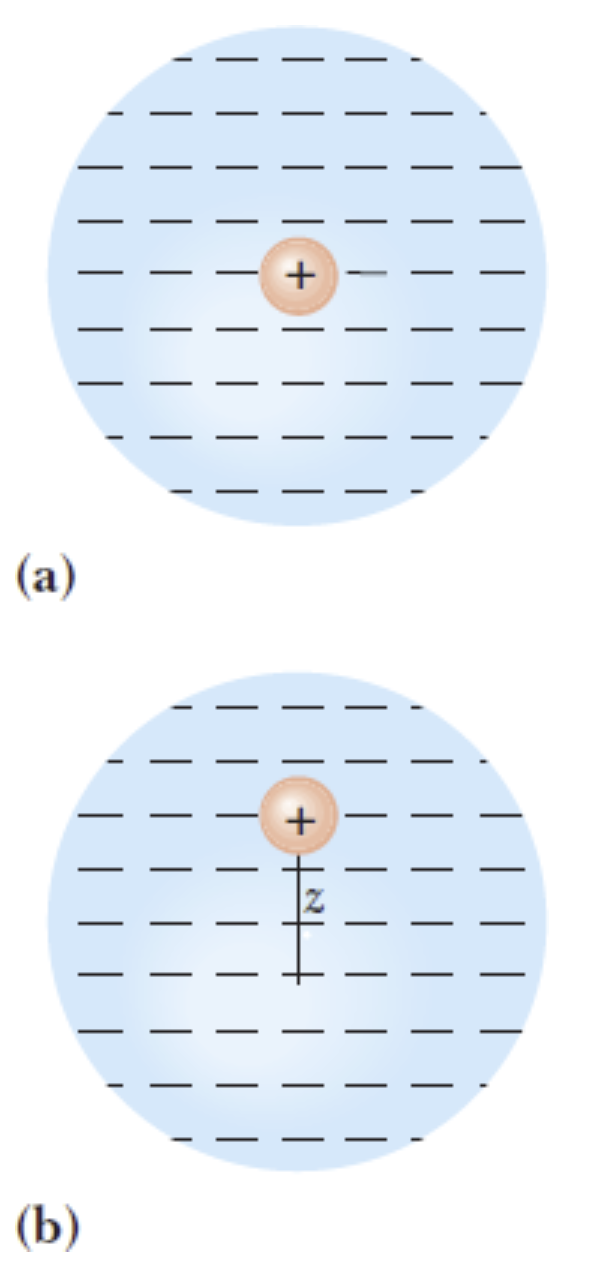
\includegraphics[width=0.25\linewidth]{figure/image70.png}
  \caption{Modello classico dell'atomo eccitato come oscillatore armonico}
  \label{fig:etichetta}
\end{figure}

Come sappiamo il modello di Bohr è stato poi superato da modelli quantistici più avanzati.\\

La \emph{luce visibile}, cui è sensibile la retina dell’occhio umano, è una particolare radiazione elettromagnetica emessa da atomi nel seguente campo di frequenze e di lunghezze d’onda (nel vuoto):

\begin{align}
    3.85 \cdot 10^{14} \leq \nu \leq 7.89 \cdot 10^{14} \ Hz\\
    2.42 \cdot 10^{15} \leq \omega \leq 4.96 \cdot 10^{15} \ \text{rad}/\text{s}\\
    0.78 \cdot 10^{-6} \geq \lambda \geq 0.38 \cdot 10^{-6} \ m
\end{align}

L’estremo superiore delle lunghezze d’onda, inferiore delle frequenze, corrisponde alla luce rossa, l’estremo inferiore delle lunghezze d’onda, superiore delle frequenze, alla luce violetta.\\

Malgrado l’impossibilità di fornire qui una spiegazione completa della radiazione di origine atomica, accenniamo lo stesso al modello classico dell’atomo come sorgente di radiazione affinché certi risultati siano utilizzabili per la comprensione almeno parziale di alcuni fenomeni.\\

Consideriamo il modello classico dell'atomo di idrogeno: un protone fermo circondato da una distribuzione sferica uniforme di carica negativa di raggio $R \sim 10^{-10}$ m. Il campo elettrico all'interno della sfera a distanza $z$ dal centro vale:

\begin{equation}
    E = \frac{\rho z}{3\varepsilon_0} = \frac{-e}{4\pi\varepsilon_0}\frac{z}{R^3} = \frac{ez}{4\pi\varepsilon_0 R^3}
\end{equation}

La forza di richiamo sull'elettrone è quindi armonica:

\begin{equation}
    F = -\frac{e^2}{4\pi\varepsilon_0 R^3}z = -Kz \quad \Rightarrow \quad \text{moto oscillatorio}
\end{equation}

con frequenza naturale:

\begin{equation}
    \omega_0 = \sqrt{\frac{K}{m_e}} = \sqrt{\frac{e^2}{4\pi\varepsilon_0 m_e R^3}} \approx 1.59 \times 10^{16}\text{ rad/s}
\end{equation}

che corrisponde a $\nu_0 \approx 2530$ THz, nel range dell'ultravioletto.\\

\subsection{Perdita di energia per irraggiamento}

La forza di reazione della radiazione su una carica oscillante vale:

\begin{equation}
    F_{\text{rad}} = \frac{\mu_0 q^2}{6\pi c} \dddot{z}
\end{equation}

Per oscillazioni quasi-monocromatiche $z \sim e^{-i\omega_0 t}$, si ha $\dddot{z} \approx -\omega_0^2\dot{z}$, quindi la forza di reazione è proporzionale alla velocità e si comporta come uno smorzamento viscoso:

\begin{equation}
    F_{\text{rad}} \approx -m_e\gamma_0\dot{z} \quad , \quad 
    \gamma_0 = \frac{\mu_0 q^2\omega_0^2}{6\pi m_e c} = 
    \frac{2r_e\omega_0^2}{3c}
\end{equation}

L'equazione del moto dell'elettrone diventa quella di un oscillatore armonico smorzato:

\begin{equation}
    \ddot{z} + \gamma_0\dot{z} + \omega_0^2 z = 0
\end{equation}

con soluzione:

\begin{equation}
    z(t) = z_0 e^{-\gamma_0 t/2}\cos(\omega' t) \quad , \quad \omega' = \sqrt{\omega_0^2 - \frac{\gamma_0^2}{4}} \approx \omega_0
\end{equation}

dove nell'ultima approssimazione abbiamo usato $\gamma_0 \ll \omega_0$, che si verifica essere $\gamma_0/\omega_0 \sim r_e/\lambda \sim 10^{-8}$.
Questa è l'\emph{approssimazione adiabatica}: il sistema perde energia molto lentamente rispetto al periodo di oscillazione. \mkeyword{approssimazione adiabatica}\\

L'energia meccanica del sistema decade quindi esponenzialmente:

\begin{tcolorbox}[colback=yellow!10!white, colframe=orange!70!black, boxrule=0.8pt]
\begin{equation}
    U(t) = \frac{1}{2}m_e\omega_0^2 z_0^2 e^{-\gamma_0 t} = U_0 e^{-t/\tau}
\end{equation}
\end{tcolorbox}

con tempo caratteristico di decadimento:

\begin{tcolorbox}[colback=yellow!10!white, colframe=orange!70!black, boxrule=0.8pt]
\begin{equation}
    \tau = \frac{1}{\gamma_0} = \frac{3c}{2r_e\omega_0^2} \approx 0.6 \text{ ns}
\end{equation}
\end{tcolorbox}

L'atomo emette quindi un pacchetto d'onda di durata $\sim\tau$, con larghezza spettrale associata:

\begin{equation}
    \Delta\nu = \frac{1}{2\pi\tau} \quad \Rightarrow \quad \frac{\Delta\nu}{\nu_0} = \frac{1}{2\pi\tau\nu_0} \approx 1.3\times10^{-7}
\end{equation}

Questo modello riproduce correttamente gli ordini di grandezza delle emissioni atomiche. La meccanica quantistica è necessaria per una descrizione precisa dei livelli energetici e delle frequenze di emissione, ma la fisica classica cattura bene la larghezza delle righe spettrali.

\subsection{Diffusione della luce}

Secondo il modello classico dell'atomo come oscillatore, quando un campo elettrico $\mathbf{E}$ variabile sinusoidalmente nel tempo, quale è quello associato a un'onda elettromagnetica armonica, agisce sull'atomo, l'equazione del moto diventa 

\begin{equation}
    m_e\ddot{z} + m_e\omega_0^2 z = eE_0 e^{-i\omega t}
\end{equation}

La soluzione \emph{stazionaria} è $z = z_0 e^{-i\omega t}$ con:

\begin{equation}
    z_0 = \frac{eE_0}{m_e(\omega_0^2 - \omega^2)}
\end{equation}

Il momento di dipolo indotto è $p_0 = ez_0 = \varepsilon_0\alpha_e E_0$, dove abbiamo definito la \emph{polarizzabilità elettronica} come: \mkeyword{polarizzabilità elettronica}

\begin{equation}
    \alpha_e = \frac{e^2}{\varepsilon_0 m_e(\omega_0^2 - \omega^2)}
\end{equation}

La potenza diffusa si ricava dalla \eqref{eq: potenza_dipolo_elettrico}:

\begin{equation}
    \langle P \rangle = \frac{\mu_0\omega^4}{12\pi c}p_0^2 = \frac{\mu_0\omega^4\varepsilon_0^2\alpha_e^2 E_0^2}{12\pi c}
\end{equation}

Per $\omega \ll \omega_0$ (luce visibile con $\omega_0$ nel range UV): $\alpha_e \approx e^2/(\varepsilon_0 m_e\omega_0^2)$ è costante e si ottiene la \emph{legge di Rayleigh}: \mkeyword{legge di Rayleigh}

\begin{tcolorbox}[colback=yellow!10!white, colframe=orange!70!black, boxrule=0.8pt]
\begin{equation}
    \langle P(\omega) \rangle \propto \omega^4 \propto \lambda^{-4}
\end{equation}
\end{tcolorbox}

Il rapporto tra la potenza diffusa dalla luce nel violetto ($\lambda \approx 380$ nm) e nel rosso ($\lambda \approx 780$ nm) vale:

\begin{equation}
    \frac{P_{\text{violetto}}}{P_{\text{rosso}}} = \left(\frac{\lambda_{\text{rosso}}}{\lambda_{\text{violetto}}}\right)^4 = \left(\frac{780}{380}\right)^4 \approx 18
\end{equation}

La luce viola e blu viene diffusa molto più efficacemente. Questo spiega due fenomeni familiari:

\begin{itemize}
    \item \textbf{Il cielo è azzurro}: la luce solare viene diffusa dall'atmosfera in tutte le direzioni e la componente blu/viola domina nell'irraggiamento diffuso.

    \item \textbf{Il tramonto è rosso}: la luce del sole al tramonto attraversa uno strato d'aria molto più spesso a causa dell'inclinazione; la componente blu viene quasi completamente diffusa via e rimane il rosso.
\end{itemize}

% \newpage

% .

% \newpage 



% In questo capitolo sfruttiamo i risultati ottenuti nel capitolo precedente
% per studiare il trasporto di energia da parte dei campi elettromagnetici
% generati da sorgenti oscillanti o in moto accelerato. Il punto di partenza
% sono i campi di radiazione ricavati per il dipolo elettrico oscillante
% \eqref{eq: E_rad_dipolo}--\eqref{eq: B_rad_dipolo}.

% \section{Potenza irradiata dal dipolo elettrico oscillante}

% \subsection{Vettore di Poynting nella zona di radiazione}

% Nella zona di radiazione ($r \gg \lambda$) i campi del dipolo elettrico
% oscillante sono:

% \begin{align}
%     \mathbf{E}_{\text{rad}} &= \frac{1}{4\pi\varepsilon_0 c^2}
%     \frac{(\ddot{\mathbf{p}}_r \times \hat{r}) \times \hat{r}}{r}
%     \label{eq: E_rad_cap} \\[6pt]
%     \mathbf{B}_{\text{rad}} &= \frac{\mu_0}{4\pi c}
%     \frac{\ddot{\mathbf{p}}_r \times \hat{r}}{r}
%     \label{eq: B_rad_cap}
% \end{align}

% Il vettore di Poynting è:

% \begin{equation}
%     \mathbf{S} = \frac{1}{\mu_0}(\mathbf{E}_{\text{rad}} \times
%     \mathbf{B}_{\text{rad}})
% \end{equation}

% Per calcolarlo esplicitamente, notiamo che dalla \eqref{eq: B_rad_cap}
% si ha $\mathbf{B}_{\text{rad}} = \frac{1}{c}\hat{r} \times
% \mathbf{E}_{\text{rad}}$, quindi:

% \begin{equation}
%     \mathbf{E}_{\text{rad}} \times \mathbf{B}_{\text{rad}} =
%     \mathbf{E}_{\text{rad}} \times \left(\frac{1}{c}\hat{r} \times
%     \mathbf{E}_{\text{rad}}\right) =
%     \frac{1}{c}\left[E_{\text{rad}}^2 \hat{r} -
%     (\mathbf{E}_{\text{rad}} \cdot \hat{r})\mathbf{E}_{\text{rad}}\right]
% \end{equation}

% Poiché nella zona di radiazione $\mathbf{E}_{\text{rad}} \perp \hat{r}$
% (il campo è trasversale), il secondo termine si annulla e si ottiene:

% \begin{tcolorbox}[colback=yellow!10!white, colframe=orange!70!black,
% boxrule=0.8pt]
% \begin{equation}\label{eq: Poynting_radiazione}
%     \mathbf{S} = \frac{E_{\text{rad}}^2}{\mu_0 c} \hat{r} =
%     \frac{\mu_0}{16\pi^2 c}
%     \frac{|(\ddot{\mathbf{p}}_r \times \hat{r}) \times \hat{r}|^2}
%     {r^2} \hat{r}
% \end{equation}
% \end{tcolorbox}

% Il vettore di Poynting è diretto radialmente verso l'esterno e decade
% come $r^{-2}$, garantendo la conservazione dell'energia: il flusso
% totale attraverso una sfera di raggio $r$ qualsiasi è indipendente
% da $r$.

% \subsection{Distribuzione angolare della potenza irradiata}

% La potenza irradiata per unità di angolo solido è:

% \begin{equation}
%     \frac{dP}{d\Omega} = |\mathbf{S}| r^2 =
%     \frac{\mu_0}{16\pi^2 c}
%     |(\ddot{\mathbf{p}}_r \times \hat{r}) \times \hat{r}|^2
% \end{equation}

% Supponiamo che il dipolo oscilli lungo $\hat{z}$, ovvero
% $\mathbf{p}(t) = p(t)\hat{z}$. Calcoliamo esplicitamente il doppio
% prodotto vettoriale. In coordinate sferiche con $\hat{z}$ come asse
% polare, il versore radiale è $\hat{r} = \sin\theta\cos\phi\,\hat{x}
% + \sin\theta\sin\phi\,\hat{y} + \cos\theta\,\hat{z}$, quindi:

% \begin{equation}
%     \ddot{\mathbf{p}}_r \times \hat{r} = \ddot{p}_r\hat{z} \times \hat{r}
%     = \ddot{p}_r(\hat{z} \times \hat{r})
% \end{equation}

% Per la geometria del problema $|\hat{z} \times \hat{r}| = \sin\theta$,
% e il doppio prodotto vettoriale dà la componente di $\ddot{\mathbf{p}}_r$
% trasversale a $\hat{r}$:

% \begin{equation}
%     |(\ddot{\mathbf{p}}_r \times \hat{r}) \times \hat{r}|^2 =
%     |\ddot{p}_r|^2 \sin^2\theta
% \end{equation}

% Pertanto:

% \begin{tcolorbox}[colback=yellow!10!white, colframe=orange!70!black,
% boxrule=0.8pt]
% \begin{equation}\label{eq: distribuzione_angolare}
%     \frac{dP}{d\Omega} = \frac{\mu_0}{16\pi^2 c}
%     |\ddot{p}_r|^2 \sin^2\theta
% \end{equation}
% \end{tcolorbox}

% Questo è il caratteristico \emph{pattern di irraggiamento del dipolo}:
% \mkeyword{pattern di irraggiamento} la radiazione è massima nel piano
% equatoriale ($\theta = \pi/2$, perpendicolare all'asse del dipolo) e
% si annulla lungo l'asse del dipolo ($\theta = 0, \pi$). Il pattern ha
% la forma di un toroide attorno all'asse $z$.

% \subsection{Potenza totale irradiata}

% Integriamo la distribuzione angolare \eqref{eq: distribuzione_angolare}
% su tutto l'angolo solido $d\Omega = \sin\theta\,d\theta\,d\phi$:

% \begin{equation}
%     P = \int \frac{dP}{d\Omega}\,d\Omega =
%     \frac{\mu_0}{16\pi^2 c} |\ddot{p}_r|^2
%     \int_0^{2\pi} d\phi \int_0^{\pi} \sin^3\theta\,d\theta
% \end{equation}

% L'integrale azimutale dà $2\pi$. Per quello polare, poniamo
% $u = \cos\theta$, $du = -\sin\theta\,d\theta$:

% \begin{equation}
%     \int_0^{\pi} \sin^3\theta\,d\theta =
%     \int_{-1}^{1} (1 - u^2)\,du =
%     \left[u - \frac{u^3}{3}\right]_{-1}^{1} =
%     \frac{2}{3} + \frac{2}{3} = \frac{4}{3}
% \end{equation}

% Quindi l'integrale totale vale $2\pi \cdot \frac{4}{3} = \frac{8\pi}{3}$,
% e la potenza istantanea irradiata è:

% \begin{tcolorbox}[colback=yellow!10!white, colframe=orange!70!black,
% boxrule=0.8pt]
% \begin{equation}\label{eq: potenza_istantanea_dipolo}
%     P_i(t) = \frac{\mu_0}{6\pi c} |\ddot{\mathbf{p}}_r|^2
% \end{equation}
% \end{tcolorbox}

% \subsection{Caso monocromatico e potenza media}

% Per oscillazioni monocromatiche $\mathbf{p}(t) = \mathbf{p}_0 e^{-i\omega t}$
% (con $\mathbf{p}_0$ reale), la derivata seconda al tempo ritardato è:

% \begin{equation}
%     \ddot{\mathbf{p}}_r = -\omega^2 \mathbf{p}_0 e^{-i\omega(t-r/c)}
%     \quad \Rightarrow \quad
%     |\ddot{\mathbf{p}}_r|^2 = \omega^4 p_0^2 \cos^2\omega(t - r/c)
% \end{equation}

% La media temporale su un periodo completo vale
% $\langle\cos^2\rangle = 1/2$, quindi:

% \begin{tcolorbox}[colback=yellow!10!white, colframe=orange!70!black,
% boxrule=0.8pt]
% \begin{align}
%     \left\langle\frac{dP}{d\Omega}\right\rangle &=
%     \frac{\mu_0 \omega^4 p_0^2}{32\pi^2 c} \sin^2\theta
%     \label{eq: dP_media} \\[8pt]
%     \langle P \rangle &= \frac{\mu_0 \omega^4 p_0^2}{12\pi c}
%     \label{eq: potenza_media_dipolo}
% \end{align}
% \end{tcolorbox}

% La dipendenza $\langle P \rangle \propto \omega^4$ è fondamentale:
% le sorgenti che oscillano a frequenza più alta irraggiano molto più
% efficacemente. Vedremo nella sezione sulla diffusione della luce che
% questa dipendenza è alla base del colore del cielo.

% \section{Formula di Larmor}

% \subsection{Derivazione}

% Consideriamo un sistema fisico elementare: una carica $q$ con
% accelerazione $\mathbf{a}(t)$, descritta nell'approssimazione di
% dipolo come $\ddot{\mathbf{p}} = q\mathbf{a}$. Sostituendo nella
% \eqref{eq: potenza_istantanea_dipolo}:

% \begin{tcolorbox}[colback=yellow!10!white, colframe=orange!70!black,
% boxrule=0.8pt]
% \begin{equation}\label{eq: Larmor}
%     P = \frac{\mu_0 q^2 a^2}{6\pi c} =
%     \frac{q^2 a^2}{6\pi\varepsilon_0 c^3}
% \end{equation}
% \end{tcolorbox}

% Questa è la \emph{formula di Larmor}: \mkeyword{formula di Larmor}
% qualsiasi carica accelerata irradia energia, con potenza proporzionale
% al quadrato dell'accelerazione. La formula di Larmor ha implicazioni
% fisiche profonde: un elettrone classico in orbita attorno a un nucleo
% è continuamente accelerato centripetamente, quindi dovrebbe irraggiare
% energia e spiralare verso il nucleo in un tempo brevissimo. Questo è
% uno dei fallimenti fondamentali della fisica classica che ha portato
% allo sviluppo della meccanica quantistica.

% \subsection{Generalizzazione relativistica}

% La formula di Larmor \eqref{eq: Larmor} vale nel limite non
% relativistico $v \ll c$. La sua generalizzazione relativistica,
% ricavabile dai potenziali di Liénard-Wiechert \eqref{potenziali
% ritardati}, è:

% \begin{tcolorbox}[colback=yellow!10!white, colframe=orange!70!black,
% boxrule=0.8pt]
% \begin{equation}\label{eq: Larmor_relativistica}
%     P = \frac{\mu_0 q^2 \gamma^6}{6\pi c}
%     \left(\dot{\beta}^2 -
%     |\boldsymbol{\beta} \times \dot{\boldsymbol{\beta}}|^2\right)
% \end{equation}
% \end{tcolorbox}

% che si riduce alla \eqref{eq: Larmor} per $\beta \to 0$
% ($\gamma \to 1$, $\dot{\boldsymbol{\beta}} \to \mathbf{a}/c$).
% Distinguiamo due casi fisicamente importanti.\\

% \textbf{Accelerazione parallela alla velocità}
% ($\boldsymbol{\beta} \parallel \dot{\boldsymbol{\beta}}$,
% acceleratore lineare): il termine $|\boldsymbol{\beta} \times
% \dot{\boldsymbol{\beta}}|^2 = 0$, quindi:

% \begin{equation}
%     P_{\parallel} = \frac{\mu_0 q^2 \gamma^6}{6\pi c} \dot{\beta}^2
% \end{equation}

% Il fattore $\gamma^6$ rende le perdite per irraggiamento enormi ad
% alte energie, rappresentando uno dei limiti fondamentali degli
% acceleratori lineari relativistici.\\

% \textbf{Accelerazione perpendicolare alla velocità}
% ($\boldsymbol{\beta} \perp \dot{\boldsymbol{\beta}}$, moto circolare):
% il termine $|\boldsymbol{\beta} \times \dot{\boldsymbol{\beta}}|^2 =
% \beta^2\dot{\beta}^2$, quindi:

% \begin{equation}
%     P_{\perp} = \frac{\mu_0 q^2 \gamma^6}{6\pi c}
%     (1 - \beta^2)\dot{\beta}^2 =
%     \frac{\mu_0 q^2 \gamma^4}{6\pi c} \dot{\beta}^2
% \end{equation}

% Questo fenomeno è detto \emph{radiazione di sincrotrone}.
% \mkeyword{radiazione di sincrotrone} Il fattore $\gamma^4$ implica
% perdite proibitive ad alte energie negli acceleratori circolari.\\

% Confrontando i due casi a parità di $\dot{\beta}$ e $\gamma$:

% \begin{equation}
%     \frac{P_{\parallel}}{P_{\perp}} = \gamma^2 \gg 1
% \end{equation}

% Quindi, ad alte energie, un acceleratore lineare perde per irraggiamento
% molto più di un acceleratore circolare, il che sembra controintuitivo
% ma è un fatto sperimentalmente ben verificato.

% \section{Dipolo di antenna}

% \subsection{Generalità}

% Un \emph{dipolo di antenna} \mkeyword{dipolo di antenna} è un filo
% conduttore di lunghezza $d$ con una distribuzione di corrente
% $I(z, t) = I_A(z)e^{-i\omega t}$. Nell'approssimazione $d \ll \lambda$
% il momento di dipolo si ricava dall'integrale:

% \begin{equation}
%     p_0 = \frac{i}{\omega}\int_{-d/2}^{d/2} I_A(z)\,dz
% \end{equation}

% che segue dalla definizione $\mathbf{p} = \int \rho\mathbf{r}\,d^3r$
% e dall'equazione di continuità $\partial_z I_A = i\omega\lambda_c$,
% dove $\lambda_c$ è la densità lineare di carica.\\

% La potenza totale irradiata si ricava dalla
% \eqref{eq: potenza_media_dipolo}:

% \begin{equation}
%     \langle P \rangle = \frac{\mu_0\omega^4}{12\pi c}|p_0|^2 =
%     \frac{Z_0\omega^4}{12\pi c^2}|p_0|^2
% \end{equation}

% Si definisce la \emph{resistenza di antenna} \mkeyword{resistenza di
% antenna} come la resistenza equivalente che dissiperebbe la stessa
% potenza per effetto Joule:

% \begin{equation}
%     \langle P \rangle = \frac{1}{2}R_{\text{ant}}I_{A0}^2
%     \quad \Rightarrow \quad
%     R_{\text{ant}} = \frac{2\langle P \rangle}{I_{A0}^2}
% \end{equation}

% \subsection{Caso a: carica solo alle estremità}

% La corrente è costante lungo il filo: $I_A(z) = I_{A0}$. L'integrale
% del momento di dipolo dà:

% \begin{equation}
%     p_0 = \frac{i}{\omega}\int_{-d/2}^{d/2} I_{A0}\,dz =
%     \frac{iI_{A0}d}{\omega}
% \end{equation}

% quindi $|p_0|^2 = I_{A0}^2 d^2/\omega^2$ e la potenza vale:

% \begin{equation}
%     \langle P \rangle = \frac{Z_0\omega^4}{12\pi c^2}
%     \frac{I_{A0}^2 d^2}{\omega^2} =
%     \frac{Z_0\omega^2 d^2}{12\pi c^2} I_{A0}^2
% \end{equation}

% La resistenza di antenna risulta:

% \begin{tcolorbox}[colback=yellow!10!white, colframe=orange!70!black,
% boxrule=0.8pt]
% \begin{equation}
%     R_{\text{ant}} = \frac{Z_0\omega^2 d^2}{6\pi c^2} =
%     \frac{2\pi Z_0}{3}\left(\frac{d}{\lambda}\right)^2
% \end{equation}
% \end{tcolorbox}

% \subsection{Caso b: corrente triangolare}

% La distribuzione di corrente si annulla alle estremità linearmente:
% $I_A(z) = I_{A0}(1 - 2|z|/d)$. L'integrale vale:

% \begin{equation}
%     \int_{-d/2}^{d/2} I_{A0}\left(1 - \frac{2|z|}{d}\right)dz =
%     2I_{A0}\int_0^{d/2}\left(1 - \frac{2z}{d}\right)dz =
%     2I_{A0}\left[\frac{d}{2} - \frac{d}{4}\right] =
%     \frac{I_{A0}d}{2}
% \end{equation}

% quindi $p_0 = iI_{A0}d/(2\omega)$, cioè la metà del caso precedente.
% Poiché la potenza scala con $|p_0|^2$, risulta un quarto:

% \begin{tcolorbox}[colback=yellow!10!white, colframe=orange!70!black,
% boxrule=0.8pt]
% \begin{equation}
%     R_{\text{ant}} = \frac{\pi Z_0}{6}\left(\frac{d}{\lambda}\right)^2
%     \approx 197\,\Omega\left(\frac{d}{\lambda}\right)^2
% \end{equation}
% \end{tcolorbox}

% \subsection{Caso c: onda stazionaria con nodi alle estremità ($d = \lambda/2$)}

% La distribuzione di corrente è sinusoidale con nodi alle estremità:
% $I_A(z) = I_{A0}\sin(k(d/2 - |z|))$. Questo è il caso dell'antenna
% a mezza lunghezza d'onda, la geometria più comune nelle applicazioni
% pratiche.\\

% Calcoliamo l'integrale del momento di dipolo con $k = \omega/c$:

% \begin{equation}
%     \int_{-d/2}^{d/2} I_{A0}\sin\left(k\left(\frac{d}{2} -
%     |z|\right)\right)dz =
%     2I_{A0}\int_0^{d/2}\sin\left(k\left(\frac{d}{2} - z\right)\right)dz
% \end{equation}

% Con la sostituzione $u = k(d/2 - z)$, $du = -k\,dz$:

% \begin{equation}
%     = \frac{2I_{A0}}{k}\int_0^{kd/2}\sin(u)\,du =
%     \frac{2I_{A0}}{k}[-\cos u]_0^{kd/2} =
%     \frac{2I_{A0}}{k}(1 - \cos(kd/2))
% \end{equation}

% Per $d = \lambda/2$, si ha $kd/2 = \pi/2$, quindi $\cos(kd/2) = 0$ e:

% \begin{equation}
%     \int_{-d/2}^{d/2} I_A(z)\,dz = \frac{2I_{A0}}{k} =
%     \frac{2I_{A0}c}{\omega}
% \end{equation}

% Il momento di dipolo è $p_0 = \frac{i}{\omega} \cdot
% \frac{2I_{A0}c}{\omega} = \frac{2iI_{A0}c}{\omega^2}$, e la potenza vale:

% \begin{equation}
%     \langle P \rangle = \frac{Z_0\omega^4}{12\pi c^2} \cdot
%     \frac{4I_{A0}^2 c^2}{\omega^4} = \frac{Z_0}{3\pi}I_{A0}^2
% \end{equation}

% La resistenza di antenna per l'antenna a $\lambda/2$ è:

% \begin{tcolorbox}[colback=yellow!10!white, colframe=orange!70!black,
% boxrule=0.8pt]
% \begin{equation}
%     R_{\text{ant}} = \frac{2Z_0}{3\pi} \approx 80\,\Omega
% \end{equation}
% \end{tcolorbox}

% Il valore $R \approx 80\,\Omega$ è un risultato fondamentale
% dell'ingegneria delle antenne: un'antenna a dipolo di mezza lunghezza
% d'onda ha una resistenza di antenna di circa $80\,\Omega$,
% indipendentemente dalla frequenza di operazione.

% \section{Modello classico dell'atomo e irraggiamento atomico}

% \subsection{Modello dell'atomo di idrogeno}

% Consideriamo il modello classico dell'atomo di idrogeno: un protone
% fermo circondato da una distribuzione sferica uniforme di carica
% negativa di raggio $R \sim 10^{-10}$ m. Il campo elettrico all'interno
% della sfera a distanza $z$ dal centro vale:

% \begin{equation}
%     E = \frac{\rho z}{3\varepsilon_0} =
%     \frac{-e}{4\pi\varepsilon_0}\frac{z}{R^3} =
%     \frac{ez}{4\pi\varepsilon_0 R^3}
% \end{equation}

% La forza di richiamo sull'elettrone è quindi armonica:

% \begin{equation}
%     F = -\frac{e^2}{4\pi\varepsilon_0 R^3}z = -Kz
%     \quad \Rightarrow \quad \text{moto oscillatorio}
% \end{equation}

% con frequenza naturale:

% \begin{equation}
%     \omega_0 = \sqrt{\frac{K}{m_e}} =
%     \sqrt{\frac{e^2}{4\pi\varepsilon_0 m_e R^3}}
%     \approx 1.59 \times 10^{16}\text{ rad/s}
% \end{equation}

% che corrisponde a $\nu_0 \approx 2530$ THz, nel range dell'ultravioletto.\\

% \subsection{Perdita di energia per irraggiamento}

% Se $z_0$ è l'ampiezza di oscillazione, il momento di dipolo vale
% $p_0 = ez_0$ e l'energia meccanica del sistema è:

% \begin{equation}
%     U = \frac{1}{2}m_e\omega_0^2 z_0^2
% \end{equation}

% La potenza media irradiata per la formula di Larmor
% \eqref{eq: Larmor} con $\langle a^2 \rangle = \omega_0^4 z_0^2/2$:

% \begin{equation}
%     \langle P \rangle = \frac{\mu_0 q^2}{6\pi c}
%     \frac{\omega_0^4 z_0^2}{2} =
%     \frac{e^2\omega_0^4 z_0^2}{12\pi\varepsilon_0 c^3}
% \end{equation}

% Introduciamo il \emph{raggio classico dell'elettrone}:
% \mkeyword{raggio classico dell'elettrone}

% \begin{tcolorbox}[colback=yellow!10!white, colframe=orange!70!black,
% boxrule=0.8pt]
% \begin{equation}
%     r_e = \frac{e^2}{4\pi\varepsilon_0 m_e c^2} \approx 2.8\text{ fm}
% \end{equation}
% \end{tcolorbox}

% In termini di $r_e$ la potenza si riscrive come:

% \begin{equation}
%     \langle P \rangle =
%     \frac{2r_e\omega_0^2}{3c} \cdot
%     \frac{1}{2}m_e\omega_0^2 z_0^2 =
%     \frac{2r_e\omega_0^2}{3c} U
% \end{equation}

% La perdita di energia per irraggiamento soddisfa l'equazione
% differenziale:

% \begin{equation}
%     \frac{dU}{dt} = -\langle P \rangle = -\frac{2r_e\omega_0^2}{3c} U
% \end{equation}

% con soluzione $U(t) = U_0 e^{-t/\tau}$ e tempo caratteristico:

% \begin{tcolorbox}[colback=yellow!10!white, colframe=orange!70!black,
% boxrule=0.8pt]
% \begin{equation}
%     \tau = \frac{3c}{2r_e\omega_0^2} \approx 0.6\text{ ns}
% \end{equation}
% \end{tcolorbox}

% L'atomo emette quindi un pacchetto d'onda di durata $\sim\tau$. La
% larghezza spettrale associata è:

% \begin{equation}
%     \Delta\nu = \frac{1}{2\pi\tau}
%     \quad \Rightarrow \quad
%     \frac{\Delta\nu}{\nu_0} = \frac{1}{2\pi\tau\nu_0} \approx
%     1.3 \times 10^{-7}
% \end{equation}

% Questo modello riproduce correttamente gli ordini di grandezza delle
% emissioni atomiche. La meccanica quantistica è necessaria per una
% descrizione precisa dei livelli energetici e delle frequenze di
% emissione, ma la fisica classica cattura bene la larghezza delle righe
% spettrali.

% \section{Diffusione della luce}

% \subsection{Scattering di Thomson}

% Consideriamo un elettrone \emph{libero} investito da un'onda
% elettromagnetica piana monocromatica con campo elettrico
% $\mathbf{E} = \mathbf{E}_0 e^{-i\omega t}$ (trascuriamo la forza
% magnetica di Lorentz in quanto di ordine $v/c$ rispetto a quella
% elettrica). L'equazione del moto dell'elettrone è:

% \begin{equation}
%     m_e\ddot{\mathbf{r}} = e\mathbf{E}_0 e^{-i\omega t}
%     \quad \Rightarrow \quad
%     \mathbf{a} = \frac{e\mathbf{E}_0}{m_e}e^{-i\omega t}
% \end{equation}

% con $\langle a^2\rangle = e^2 E_0^2/(2m_e^2)$. Per la formula di
% Larmor la potenza diffusa è:

% \begin{equation}
%     P_{\text{diff}} = \frac{\mu_0 e^2}{6\pi c}\langle a^2\rangle =
%     \frac{\mu_0 e^2}{6\pi c} \cdot \frac{e^2 E_0^2}{2m_e^2} =
%     \frac{\mu_0 e^4 E_0^2}{12\pi m_e^2 c}
% \end{equation}

% L'intensità dell'onda incidente è:

% \begin{equation}
%     I_0 = \langle|\mathbf{S}|\rangle =
%     \frac{1}{2}\varepsilon_0 c E_0^2 =
%     \frac{E_0^2}{2\mu_0 c}
% \end{equation}

% La \emph{sezione d'urto di diffusione} \mkeyword{sezione d'urto di
% diffusione} è definita come il rapporto tra potenza diffusa e
% intensità incidente, e ha le dimensioni di un'area:

% \begin{equation}
%     \sigma_T = \frac{P_{\text{diff}}}{I_0} =
%     \frac{\mu_0 e^4 E_0^2}{12\pi m_e^2 c} \cdot
%     \frac{2\mu_0 c}{E_0^2} =
%     \frac{\mu_0^2 e^4}{6\pi m_e^2}
% \end{equation}

% Riscrivendo in termini del raggio classico dell'elettrone
% $r_e = \mu_0 e^2/(4\pi m_e)$:

% \begin{tcolorbox}[colback=yellow!10!white, colframe=orange!70!black,
% boxrule=0.8pt]
% \begin{equation}\label{eq: sezione_urto_Thomson}
%     \sigma_T = \frac{8\pi}{3}r_e^2 \approx 0.66\times10^{-28}\text{ m}^2
% \end{equation}
% \end{tcolorbox}

% Questa è la \emph{sezione d'urto di Thomson}. \mkeyword{sezione d'urto
% di Thomson} Notare che $\sigma_T$ non dipende da $\omega$: un elettrone
% libero diffonde tutte le frequenze con la stessa efficienza. L'unità
% $10^{-28}$ m$^2 = 10^{-24}$ cm$^2$ prende il nome di \emph{barn}
% \mkeyword{barn} ed è l'unità standard in fisica nucleare e delle
% particelle. Questo risultato descrive correttamente la diffusione per
% $h\nu \ll m_e c^2$ (cioè $\nu \lesssim 10^{20}$ Hz); a energie più
% alte entrano in gioco effetti quantistici descritti dalla sezione
% d'urto di Klein-Nishina.

% \subsection{Diffusione di Rayleigh}

% Per la diffusione da atomi, l'elettrone non è libero ma legato con
% frequenza di risonanza $\omega_0$. L'equazione del moto diventa:

% \begin{equation}
%     m_e\ddot{z} + m_e\omega_0^2 z = eE_0 e^{-i\omega t}
% \end{equation}

% La soluzione stazionaria è $z = z_0 e^{-i\omega t}$ con:

% \begin{equation}
%     z_0 = \frac{eE_0/m_e}{\omega_0^2 - \omega^2}
% \end{equation}

% Il momento di dipolo indotto è $p_0 = ez_0 = \varepsilon_0\alpha_e E_0$,
% dove la \emph{polarizzabilità elettronica} vale:
% \mkeyword{polarizzabilità elettronica}

% \begin{equation}
%     \alpha_e = \frac{e^2}{\varepsilon_0 m_e(\omega_0^2 - \omega^2)}
% \end{equation}

% La potenza diffusa si ricava dalla \eqref{eq: potenza_media_dipolo}:

% \begin{equation}
%     \langle P \rangle = \frac{\mu_0\omega^4}{12\pi c}p_0^2 =
%     \frac{\mu_0\omega^4\varepsilon_0^2\alpha_e^2 E_0^2}{12\pi c}
% \end{equation}

% La sezione d'urto di Rayleigh è quindi:

% \begin{equation}
%     \sigma_R = \frac{\langle P\rangle}{I_0} =
%     \frac{\mu_0\omega^4\varepsilon_0^2\alpha_e^2 E_0^2}{12\pi c} \cdot
%     \frac{2}{  \varepsilon_0 c E_0^2} \propto \omega^4\alpha_e^2
% \end{equation}

% Per $\omega \ll \omega_0$ (luce visibile con $\omega_0$ nel range UV):
% $\alpha_e \approx e^2/(\varepsilon_0 m_e\omega_0^2)$ è costante e si
% ottiene la \emph{legge di Rayleigh}: \mkeyword{legge di Rayleigh}

% \begin{tcolorbox}[colback=yellow!10!white, colframe=orange!70!black,
% boxrule=0.8pt]
% \begin{equation}
%     \sigma_R \propto \omega^4 \propto \lambda^{-4}
% \end{equation}
% \end{tcolorbox}

% Il rapporto tra luce diffusa nel violetto ($\lambda \approx 380$ nm)
% e nel rosso ($\lambda \approx 780$ nm) vale:

% \begin{equation}
%     \frac{\sigma_{\text{violetto}}}{\sigma_{\text{rosso}}} =
%     \left(\frac{\lambda_{\text{rosso}}}{\lambda_{\text{violetto}}}
%     \right)^4 = \left(\frac{780}{380}\right)^4 \approx 7\div 10
% \end{equation}

% La luce viola e blu viene diffusa molto più efficacemente. Questo
% spiega due fenomeni familiari:

% \begin{itemize}
%     \item \textbf{Il cielo è azzurro}: la luce solare viene diffusa
%     dall'atmosfera in tutte le direzioni e la componente blu/viola
%     domina nell'irraggiamento diffuso.

%     \item \textbf{Il tramonto è rosso}: la luce del sole attraversa
%     uno strato d'aria molto più spesso; la componente blu viene
%     quasi completamente diffusa via e rimane il rosso.
% \end{itemize}

% \subsection{Polarizzazione della luce diffusa}

% Nella zona di radiazione il campo $\mathbf{E}_{\text{rad}}$ è
% proporzionale alla componente di $\ddot{\mathbf{p}}_r$ trasversale
% a $\hat{r}$, ovvero $\mathbf{E}_{\text{rad}} \propto
% (\ddot{\mathbf{p}}_r \times \hat{r}) \times \hat{r} =
% \ddot{\mathbf{p}}_{r,\perp}$.\\

% Consideriamo un'onda incidente lungo $\hat{z}$ con polarizzazione
% lungo $\hat{x}$: il dipolo indotto oscilla lungo $\hat{x}$. La luce
% diffusa nella direzione $\hat{y}$ (perpendicolare a $\hat{z}$ e
% $\hat{x}$) ha la componente di $\ddot{\mathbf{p}}$ trasversale a
% $\hat{y}$ che è tutta lungo $\hat{x}$: la luce è
% \emph{completamente polarizzata linearmente} lungo $\hat{x}$.\\

% Per luce incidente non polarizzata, la media sulle polarizzazioni dà luce diffusa a $90°$ \emph{parzialmente polarizzata}. 
% Questo effetto è osservabile guardando il cielo con un filtro polarizzatore: in direzione perpendicolare al sole, la luce è parzialmente polarizzata.